\documentclass{article}

\usepackage{graphicx}
\usepackage{tikz}
\usepackage{tikzsymbols}
\usetikzlibrary{calc,patterns,shapes.geometric}
\pagestyle{empty}
\usepackage[margin=0pt]{geometry}
\geometry{papersize={14in,12in}}

\def\centerarc[#1](#2)(#3:#4:#5){\draw[#1] ($(#2)+({#5*cos(#3)},{#5*sin(#3)})$) arc (#3:#4:#5);}

\begin{document}
	\begin{figure}
		\centering
		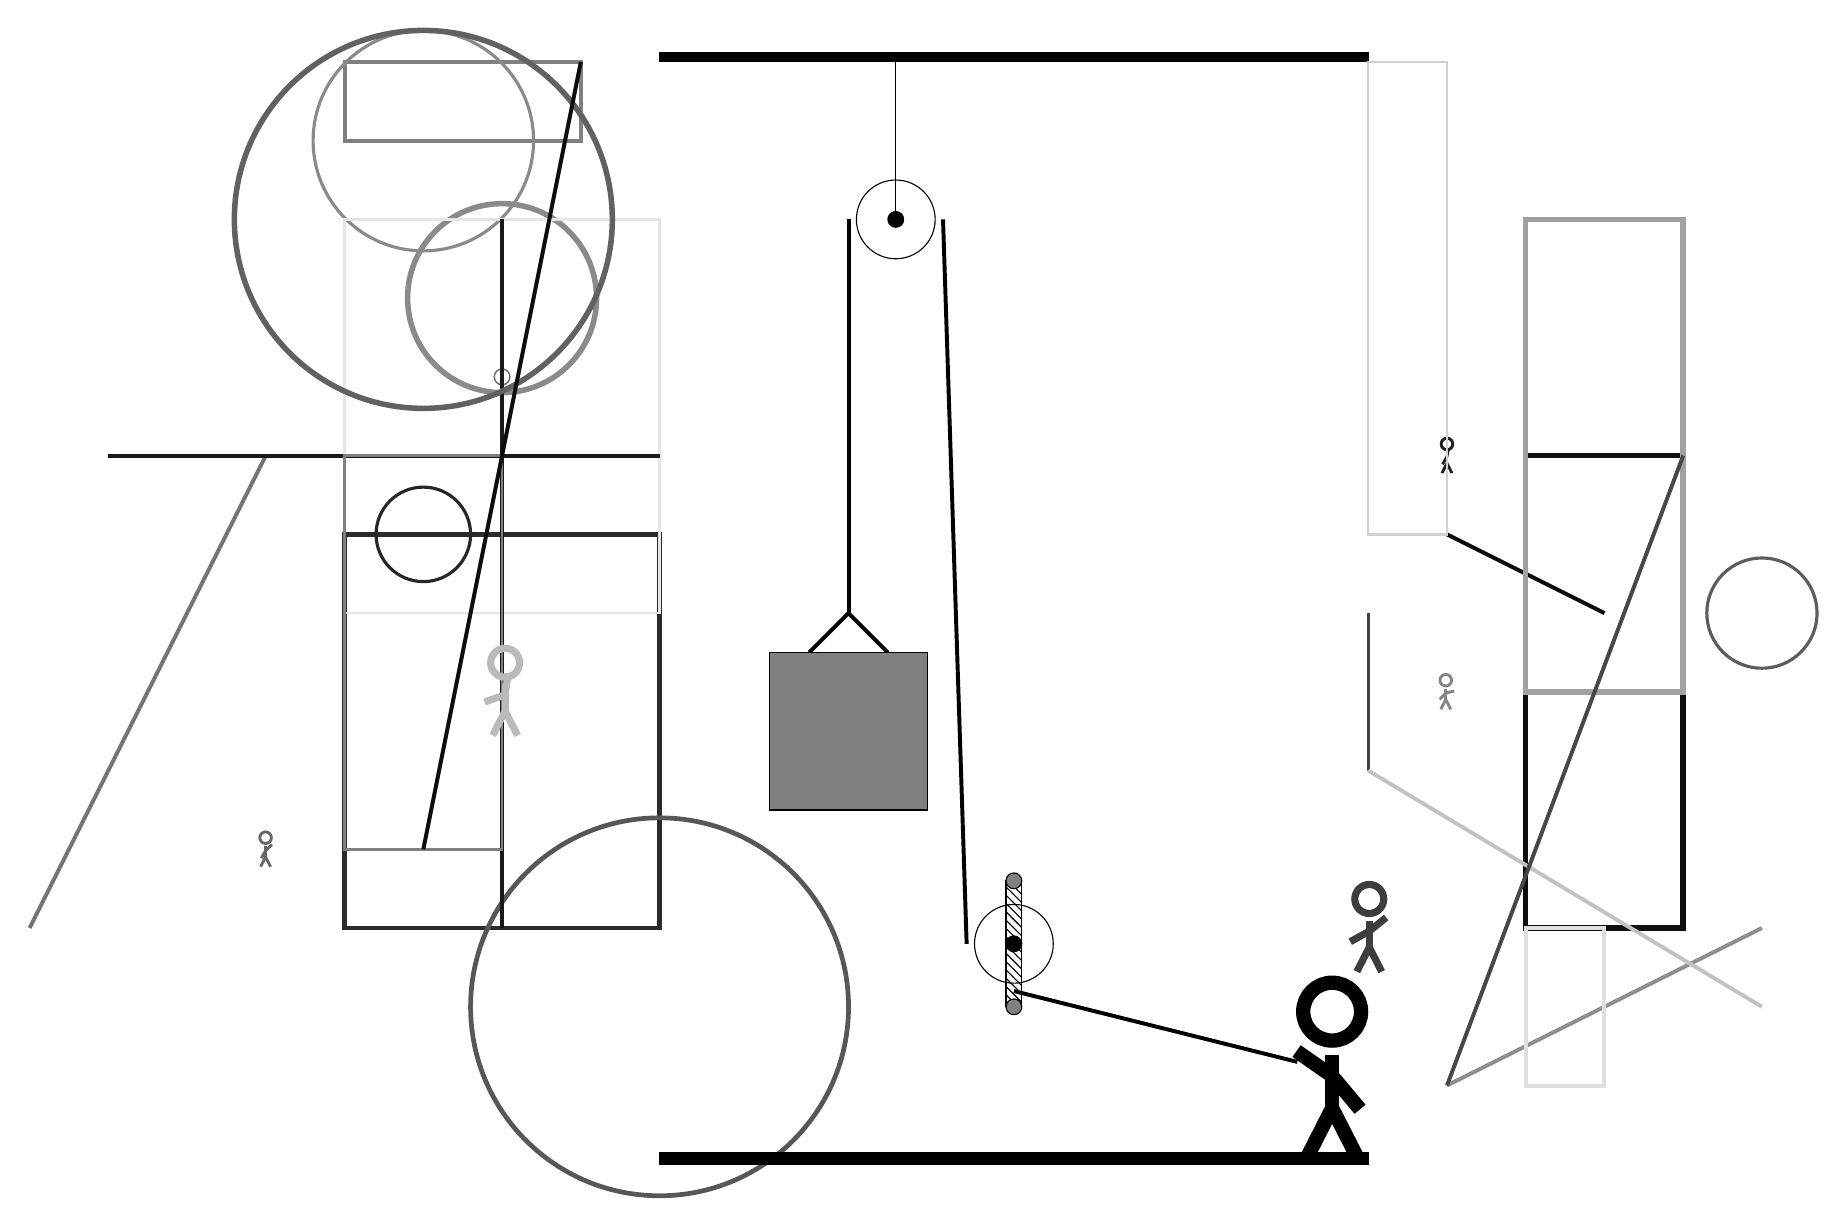
\begin{tikzpicture}
			%%%%% START %%%%%
			
			\draw[fill=black] (-2, 14) rectangle (7, 14.125);
			
			\draw[line width=0.5mm, color=black!50] (-3, 13) rectangle (-6, 14);
			
			\draw[line width=0.4mm, color=black!74] (7, 7) rectangle (7, 5);
			\draw [line width=0.2mm, color=black!55](-4, 10) circle (0.1);
			\node[line width=0.3mm, color=black!60] at (-7, 4) {\Strichmaxerl[2][61][43]};
			\node[line width=0.7mm, color=black!76] at (7, 3) {\Strichmaxerl[5][29][39]};
			\draw[line width=0.6mm, color=black!83] (-2, 8) rectangle (-6, 3);
			\draw [line width=0.6mm, color=black!66](-2, 2) circle (2.4);
			\draw[line width=0.7mm, color=black!94] (9, 9) rectangle (11, 3);
			\draw[line width=0.5mm, color=black!44](12, 3) -- (8, 1);
			\draw[line width=0.5mm, color=black!98](8, 8) -- (10, 7);
			\draw[line width=0.5mm, color=black!55](-7, 9) -- (-10, 3);
			\draw[line width=0.5mm, color=black!24](12, 2) -- (7, 5);
			\draw [line width=0.7mm, color=black!46](-4, 11) circle (1.2);
			
			\node[line width=0.4mm, color=black!88] at (8, 9) {\Strichmaxerl[2][59][80]};
			\draw [line width=0.4mm, color=black!46](-5, 13) circle (1.4);
			\draw[line width=0.5mm, color=black!13] (9, 3) rectangle (10, 1);
			
			\draw [line width=0.4mm, color=black!64](12, 7) circle (0.7);
			
			\node[line width=0.5mm, color=black!48] at (8, 6) {\Strichmaxerl[2][46][14]};
			\draw[line width=0.3mm, color=black!10] (-2, 7) rectangle (-6, 12);
			\draw[line width=0.5mm, color=black!90](-4, 3) -- (-4, 12);
			\draw [line width=0.7mm, color=black!62](-5, 12) circle (2.4);
			
			\draw[line width=0.7mm, color=black!37] (9, 12) rectangle (11, 6);
			\draw[line width=0.3mm, color=black!18] (8, 14) rectangle (7, 8);
			\draw[line width=0.5mm, color=black!90](-2, 9) -- (-9, 9);
			\draw[line width=0.3mm, color=black!50] (-4, 4) rectangle (-6, 9);
			\draw[line width=0.5mm, color=black!72](11, 9) -- (8, 1);
			\node[line width=0.6mm, color=black!27] at (-4, 6) {\Strichmaxerl[5][19][82]};
			\draw [line width=0.4mm, color=black!85](-5, 8) circle (0.6);
			
			\draw[line width=0.5mm, color=black!95](-3, 14) -- (-5, 4);
			
			
			\draw (1, 12) circle (0.5);
			\draw[fill=black] (1, 12) circle (0.1);
			\draw (1, 14) -- (1, 12);
			
			\draw[fill=white](2.5, 2.8) circle (0.5);
			\draw[fill=black] (2.5, 2.8) circle (0.1);
			\draw[pattern=north west lines, pattern color=black] (2.4, 3.6) rectangle (2.6, 2.0);
			\draw[fill=black!50] (2.5, 3.6) circle (0.1);
			\draw[fill=black!50] (2.5, 2.0) circle (0.1);
			
			\draw[line width=0.5mm] (-0.1, 6.5) -- (0.4, 7.0) -- (0.9, 6.5);
			\draw[fill=black!50] (-0.6, 6.5) rectangle (1.4, 4.5);
			
			\draw[line width=0.5mm] (0.4, 12) -- (0.4, 7.0);
			\centerarc[line width=0.5mm](1, 12)(0:180:0.6);
			\draw[line width=0.5mm](1.6, 12) -- (1.9, 2.8);
			\centerarc[line width=0.5mm](2.5, 2.8)(180:270:0.6);
			\draw[line width=0.5mm](2.5, 2.2) -- (6.1, 1.3);
			
			\node at (6.5, 1.2) {\Strichmaxerl[10][-35][-50]};
			
			\draw[fill=black] (-2, 0) rectangle (7, 0.15);
			
			%%%%% END %%%%%
		\end{tikzpicture}
	\end{figure}	
\end{document}